% ch09a Screening and plasmons, part a (书页 115-137 / 分册p001-023；9.4节止于书137上部，9.5起见 ch09b)
% 第9章 Screening and plasmons
\chapter{屏蔽与等离激元}

在 $T_{\mathrm{k}}$ 以下对局域磁矩的屏蔽（screening）是近藤问题的本质。一个远没有那么奇特的屏蔽例子，是往电子气中引入一个正电荷 $Q$。为了在正电荷所在处恢复电中性，电子会将这个电荷屏蔽掉，从而削弱它的净电场。事实上，无论试探电荷带何种符号，屏蔽都会发生。之所以如此，是因为电子在电子气中运动时，并不需要把所有其他电子都推开。电子气中所有电子之间的相互排斥为电子的运动清出了通路。其结果是，电子之间的有效相互作用从长程的库仑 $1/r$ 被削弱为短程得多的相互作用。在托马斯–费米层次上，新的相互作用呈指数衰减。虽然这种相互作用高估了屏蔽的效应，但它确实说明了排斥相互作用屏蔽电子气中电子的效率之高。

\section{托马斯–费米屏蔽}

设电荷 $Q$ 位于原点。在没有电子气时，距原点 $r$ 处的电子感受到电势 $\phi=Q/r$，相应的势能为
\begin{equation*}
U=-e\phi=-e\frac{Q}{r}.\tag{9.1}
\end{equation*}
当电子气存在时，电荷 $Q$ 周围的电势将受到屏蔽。物理上，屏蔽电荷由有电荷 $Q$ 时电子气的电荷密度与无外电荷时的电荷密度之差决定。令 $-e\delta n(\mathbf{r})$ 表示这个差。对总电荷分布的泊松方程
\begin{equation*}
-\nabla^2\phi_{\mathrm{eff}}(\mathbf{r})=4\pi\left[Q\delta(\mathbf{r})-e\delta n(\mathbf{r})\right],\tag{9.2}
\end{equation*}
同时依赖于 $Q$ 与屏蔽电荷 $-e\delta n(\mathbf{r})$，其中 $\phi_{\mathrm{eff}}$ 是电荷 $Q$ 在电子气中的真实电势。求解式 (9.2) 的最简单办法是傅里叶变换。我们定义
\begin{equation*}
f(\mathbf{k})=\int\mathrm{d}\mathbf{r}\,\mathrm{e}^{-\mathrm{i}\mathbf{k}\cdot\mathbf{r}}f(\mathbf{r}).\tag{9.3}
\end{equation*}
于是
\begin{equation*}
k^2U_{\mathrm{eff}}(\mathbf{k})=-4\pi eQ+4\pi e^2\delta n(\mathbf{k}).\tag{9.4}
\end{equation*}
求解这个精确方程需要对屏蔽电荷作某种拟设（ansatz）。最简单的近似是托马斯（T1927）与费米（F1928）的近似：假定电子气对电荷 $Q$ 的响应就好像它在局域上是自由电子气一样。物理上，这一假设意味着电势是在费米波长所设定的距离尺度上缓变的函数。其净效果是化学势发生形式为 $\mu\to\mu+U_{\mathrm{eff}}(\mathbf{r})$ 的移动。让我们定义一个新的单粒子能级
\begin{equation*}
\epsilon_{\mathbf{k}}(\mathbf{r})=\frac{\hbar^2k^2}{2m}+U_{\mathrm{eff}}(\mathbf{r}).\tag{9.5}
\end{equation*}
有效的费米–狄拉克分布函数是
\begin{equation*}
n_{\mathbf{k}}(\mathbf{r})=\frac{1}{1+\mathrm{e}^{\beta(\epsilon_{\mathbf{k}}(\mathbf{r})-\mu)}},\tag{9.6}
\end{equation*}
于是 $\mathbf{r}$ 处的有效密度为
\begin{equation*}
\begin{aligned}
\langle n(\mathbf{r})\rangle&=2\int\frac{\mathrm{d}\mathbf{k}}{(2\pi)^3}\,n_{\mathbf{k}}(\mathbf{r})\\
&=n_{\mathrm{e}}-2\beta\int\frac{\mathrm{d}\mathbf{k}}{(2\pi)^3}\,U_{\mathrm{eff}}(\mathbf{r})\,\frac{\mathrm{e}^{\beta(\epsilon_{\mathbf{k}}-\mu)}}{\left(1+\mathrm{e}^{\beta(\epsilon_{\mathbf{k}}-\mu)}\right)^2}+\cdots\\
&\simeq n_{\mathrm{e}}-\frac{\partial n_{\mathrm{e}}}{\partial\mu}\,U_{\mathrm{eff}}(\mathbf{r})+\cdots,
\end{aligned}\tag{9.7}
\end{equation*}
其中我们对分布函数作了展开，只保留 $U_{\mathrm{eff}}$ 的线性项。仅当 $\epsilon_{\mathrm{F}}\gg U_{\mathrm{eff}}(\mathbf{r})$ 时这一展开才成立。现在可以计算 $\delta n(\mathbf{r})$ 了，因为
\begin{equation*}
\delta n(\mathbf{r})=\langle n(\mathbf{r})\rangle-n_{\mathrm{e}}=-\frac{\partial n_{\mathrm{e}}}{\partial\mu}\,U_{\mathrm{eff}}(\mathbf{r}),\tag{9.8}
\end{equation*}
这意味着
\begin{equation*}
k^2U_{\mathrm{eff}}(\mathbf{k})=-4\pi e\left(Q+e\,\frac{\partial n_{\mathrm{e}}}{\partial\mu}\,U_{\mathrm{eff}}(k)\right)\tag{9.9}
\end{equation*}
或者等价地
\begin{equation*}
U_{\mathrm{eff}}(\mathbf{k})=\frac{-4\pi eQ}{k^2+4\pi e^2\,\partial n_{\mathrm{e}}/\partial\mu}.\tag{9.10}
\end{equation*}
$U_{\mathrm{eff}}(\mathbf{k})$ 的傅里叶逆变换
\begin{equation*}
\begin{aligned}
U_{\mathrm{eff}}(\mathbf{r})&=-\frac{4\pi eQ}{(2\pi)^3}\int\frac{\mathrm{e}^{\mathrm{i}\mathbf{k}\cdot\mathbf{r}}\,\mathrm{d}\mathbf{k}}{k^2+4\pi e^2\,\partial n_{\mathrm{e}}/\partial\mu}\\
&=-2\frac{eQ}{\pi r}\int_{-\infty}^{\infty}\mathrm{d}k\,\frac{k\sin kr}{k^2+4\pi e^2\,\partial n_{\mathrm{e}}/\partial\mu}\\
&=-eQ\,\frac{\mathrm{e}^{-\kappa_{\mathrm{TF}}r}}{r},
\end{aligned}\tag{9.11}
\end{equation*}
表明电荷 $Q$ 周围的电子所产生的静电势
\begin{equation*}
\phi_{\mathrm{eff}}(\mathbf{r})=-e\,\frac{\mathrm{e}^{-\kappa_{\mathrm{TF}}r}}{r},\tag{9.12}
\end{equation*}
呈指数衰减。电子气通过在一个由下式确定的长度尺度上屏蔽电荷，使裸库仑场受到衰减：
\begin{equation*}
\kappa_{\mathrm{TF}}^2=4\pi e^2\frac{\partial n_{\mathrm{e}}}{\partial\mu}.\tag{9.13}
\end{equation*}
再强调一遍，这个结果只在电子气诱导的场缓变的极限下成立。我们回忆第 2 章的
\begin{equation*}
n_{\mathrm{e}}=\left(\frac{2m\mu_0}{\hbar^2}\right)^{3/2}\frac{1}{3\pi^2},\tag{9.14}
\end{equation*}
来估计 $\kappa_{\mathrm{TF}}$。于是
\begin{equation*}
\frac{\partial n_{\mathrm{e}}}{\partial\mu_0}=\frac{3}{2}\,\frac{n_{\mathrm{e}}}{\mu_0}=\frac{3mn_{\mathrm{e}}}{p_{\mathrm{F}}^2}.\tag{9.15}
\end{equation*}
回忆 $a_0=\hbar^2/me^2$、$n_{\mathrm{e}}=p_{\mathrm{F}}^3/(3\pi^2\hbar^3)$ 以及 $r_{\mathrm{e}}=1.92\,\hbar/p_{\mathrm{F}}$，便可以化简为
\begin{equation*}
\kappa_{\mathrm{TF}}^2=\frac{12\pi me^2n_{\mathrm{e}}}{p_{\mathrm{F}}^2}=\frac{2.434}{a_0^2}\,\frac{1}{r_{\mathrm{s}}},\tag{9.16}
\end{equation*}
即托马斯–费米屏蔽长度倒数（逆屏蔽长度）的平方。回忆 $r_{\mathrm{s}}\sim 2$ 到 6。因此 $\kappa_{\mathrm{TF}}^{-1}=0.34\sqrt{r_{\mathrm{s}}}\,\text{\AA}$，介于 $0.45\,\text{\AA}$ 与 $0.9\,\text{\AA}$ 之间。虽然托马斯–费米理论预言的金属中电子屏蔽长度一般短于粒子间距，但这一结果只描述式 (9.11) 那样围绕给定电荷的电势在长距离处的衰减。该理论并不能正确处理与粒子间距相当的距离上的屏蔽。要看清短距离下的行为需要更严格的处理，我们将在后面一节中展开。

\section{等离体振荡与集体坐标}

我们发展的电子气屏蔽理论假设电子做缓慢运动。一般说来这并不成立，尤其是在与粒子间距倒数相当的大波矢处。在这个极限下，电子气的集体激发变得可以触及。这类集体激发称为等离激元（plasmon）。我们将建立等离激元的两种表述。第一种是较为传统的运动方程方法；第二种我们将回到玻姆（Bohm）与 Pines（BP1953）原创的集体坐标（collective coordinate）方法。我们将对这一技术作一综述，因为它如今已是描述集体现象的标准程序。

等离体激发的存在性可以直接从动量空间中电子密度的运动方程确立。为此，我们回忆库仑相互作用在动量空间中的形式
\begin{equation*}
\sum_{\mathbf{k}}\frac{4\pi}{k^2}\,\mathrm{e}^{\mathrm{i}\mathbf{k}\cdot(\mathbf{r}_i-\mathbf{r}_j)}=\frac{1}{|\mathbf{r}_i-\mathbf{r}_j|},\tag{9.17}
\end{equation*}
这意味着可以把电子气的哈密顿量改写为
\begin{equation*}
\begin{aligned}
H&=\sum_i\frac{p_i^2}{2m}+\frac{1}{2}\sum_{i\neq j}\sum_{\mathbf{k}}\frac{4\pi e^2}{k^2}\,\mathrm{e}^{\mathrm{i}\mathbf{k}\cdot(\mathbf{r}_i-\mathbf{r}_j)}\\
&=\sum_i\frac{p_i^2}{2m}+\sum_{\mathbf{k}}\frac{V_{\mathbf{k}}}{2}\left(n_{\mathbf{k}}n_{-\mathbf{k}}-N\right)
\end{aligned}\tag{9.18}
\end{equation*}
其中 $n_{\mathbf{k}}=\sum_i\mathrm{e}^{\mathrm{i}\mathbf{k}\cdot\mathbf{r}_i}$，$N$ 是电子数，$V_{\mathbf{k}}=4\pi e^2/k^2$。由于我们选的盒子具有单位体积，$n_{\mathbf{k}}$ 的表达式中不带 $V^{-1}$ 归一化因子。

为确定集体激发，需要 $n_{\mathbf{k}}$ 的时间演化：
\begin{equation*}
\begin{aligned}
\mathrm{i}\dot{n}_{\mathbf{k}}&=[n_{\mathbf{k}},H]/\hbar\\
&=\frac{1}{\hbar}\sum_i\left[\frac{\hbar^2}{m}\nabla_{\mathbf{r}_i}\mathrm{e}^{\mathrm{i}\mathbf{k}\cdot\mathbf{r}_i}\cdot\nabla_{\mathbf{r}_i}+\frac{\hbar^2}{2m}\nabla_{\mathbf{r}_i}^2\mathrm{e}^{\mathrm{i}\mathbf{k}\cdot\mathbf{r}_i}\right]\\
&=-\sum_i\mathrm{e}^{\mathrm{i}\mathbf{k}\cdot\mathbf{r}_i}\left(\frac{\mathbf{k}\cdot\mathbf{p}_i}{m}+\frac{\hbar k^2}{2m}\right).
\end{aligned}\tag{9.19}
\end{equation*}
二阶导数为
\begin{equation*}
\begin{aligned}
\ddot{n}_{\mathbf{k}}&=\sum_i\mathrm{e}^{\mathrm{i}\mathbf{k}\cdot\mathbf{r}_i}\left(\frac{\mathbf{k}\cdot\mathbf{p}_i}{m}+\frac{\hbar k^2}{2m}\right)^{\!2}+\frac{2\pi e^2}{\hbar}\sum_i\left[\mathrm{e}^{\mathrm{i}\mathbf{k}\cdot\mathbf{r}_i}\,\frac{\mathbf{k}\cdot\mathbf{p}_i}{m}\,,\,\sum_{\mathbf{q}}\left(\frac{n_{\mathbf{q}}^{\dagger}n_{\mathbf{q}}-N}{q^2}\right)\right]\\
&=\sum_i\mathrm{e}^{\mathrm{i}\mathbf{k}\cdot\mathbf{r}_i}\left(\frac{\mathbf{k}\cdot\mathbf{p}_i}{m}+\frac{\hbar k^2}{2m}\right)^{\!2}-\frac{4\pi e^2}{m}\sum_{\mathbf{q}}\mathbf{k}\cdot\mathbf{q}\,\frac{n_{\mathbf{k}-\mathbf{q}}n_{\mathbf{q}}}{q^2}.
\end{aligned}\tag{9.20}
\end{equation*}
我们把 $\mathbf{k}=\mathbf{q}$ 的相互作用项分离出来，它可以写成
\begin{equation*}
4\pi e^2\,\frac{k^2}{mk^2}\,n_0n_{\mathbf{k}}=\frac{4\pi e^2n_{\mathrm{e}}}{m}\,n_{\mathbf{k}}=\omega_{\mathrm{p}}^2 n_{\mathbf{k}}.\tag{9.21}
\end{equation*}
把 $\ddot{n}_{\mathbf{k}}$ 改写成如下富有启发性的形式，便可看出 $\omega_{\mathrm{p}}$ 代表电子气集体振荡的频率：
\begin{equation*}
\ddot{n}_{\mathbf{k}}+\omega_{\mathrm{p}}^2 n_{\mathbf{k}}=\sum_i\mathrm{e}^{\mathrm{i}\mathbf{k}\cdot\mathbf{r}_i}\left(\frac{\mathbf{k}\cdot\mathbf{p}_i}{m}+\frac{\hbar k^2}{2m}\right)^{\!2}-\frac{4\pi e^2}{m}\sum_{\mathbf{q}\neq\mathbf{k}}\mathbf{k}\cdot\mathbf{q}\,\frac{n_{\mathbf{k}-\mathbf{q}}n_{\mathbf{q}}}{q^2}.\tag{9.22}
\end{equation*}
于是我们看到，若式 (9.22) 右边的各项都很小，密度 $n_{\mathbf{k}}$ 便以频率 $\omega_{\mathrm{p}}$——等离体频率（plasma frequency）——振荡。第一项的量级为 $k^2v_{\mathrm{F}}^2n_{\mathbf{k}}$。在下一项中出现的是 $n_{\mathbf{q}}$ 的乘积。由于密度是诸多相位无规变化的指数项之和，可以预期第二项的贡献极小。忽略这一贡献的近似称为无规相位近似（random phase approximation）（P1963）。在这一理论层次上，若
\begin{equation*}
\omega_{\mathrm{p}}^2\gg k^2v_{\mathrm{F}}^2,\tag{9.23}
\end{equation*}
则存在一个良好定义的等离体频率。对密度 $n_{\mathrm{e}}\sim10^{23}\,\mathrm{e}^{-}/\mathrm{cm}^3$，$\omega_{\mathrm{p}}\sim10^{16}\,\mathrm{s}^{-1}$，或者等价地，等离体振荡的能量为
\begin{equation*}
\hbar\omega_{\mathrm{p}}\sim12\,\mathrm{eV}.\tag{9.24}
\end{equation*}
如此高能的激发不可能由离子的热振荡或类声子振荡产生，也不能被单个电子激发。等离体振荡，即等离激元，源于固体中全部电子的集体运动。因此，等离激元是长波长振荡。我们通过考虑比值 $\omega_{\mathrm{p}}/\kappa_{\mathrm{TF}}$ 来估计等离激元得以存在的最大波矢。回忆 $\kappa_{\mathrm{TF}}^2=4me^2p_{\mathrm{F}}/\pi\hbar^3$。于是
\begin{equation*}
\begin{aligned}
\omega_{\mathrm{p}}/\kappa_{\mathrm{TF}}&=\left(\frac{4\pi e^2n_{\mathrm{e}}}{m}\,\frac{\pi\hbar^3}{4p_{\mathrm{F}}me^2}\right)^{1/2}\\
&=\frac{p_{\mathrm{F}}}{\sqrt{3}\,m}=\frac{v_{\mathrm{F}}}{\sqrt{3}}.
\end{aligned}\tag{9.25}
\end{equation*}
我们发现 $\omega_{\mathrm{p}}\propto v_{\mathrm{F}}\kappa_{\mathrm{TF}}$。与式 (9.23) 比较可知，若 $k\ll\kappa_{\mathrm{TF}}$，则存在良好定义的等离体振荡；对 $k>\kappa_{\mathrm{TF}}$，电子各自独立行动。还要注意 $\omega_{\mathrm{p}}^2\sim1/m$。对相互作用系统，我们把 $m$ 换成有效质量 $m^{*}$。在 $m^{*}\to\infty$ 的绝缘体中，$\omega_{\mathrm{p}}$ 的大小是相互作用电子系统中绝缘体–金属转变的敏感判据。

真正证明等离激元具有良好定义激发之完整性的分析，出自玻姆与 Pines（BP1953）的集体坐标处理。这是一种极为有用的技术，正如在本书最后一章讨论莫特绝缘体、处理哈伯德模型时你将再次看到的那样。基本想法是通过扩大原来的希尔伯特空间，重新表述哈密顿量，使电子间库仑相互作用的长程部分用集体场（等离体模式）来描述。当我们用约束去掉非物理态之后，得到的哈密顿量将变成一个只带短程库仑相互作用的、与等离体振荡模式耦合的相互作用电子气。

出发点是一般的相互作用电子哈密顿量
\begin{equation*}
H=\sum_i\frac{p_i^2}{2m}+2\pi e^2\sum_{\mathbf{k},i,j}\frac{\mathrm{e}^{\mathrm{i}\mathbf{k}\cdot(\mathbf{x}_i-\mathbf{x}_j)}}{k^2}-2\pi n_{\mathrm{e}}^2\sum_k\frac{1}{k^2},
\end{equation*}
其中最后一项减去了电子的自相互作用，这一项代表均匀正电荷背景。关键想法是把这个哈密顿量换成用两个实场表述的等价哈密顿量：一个纵向矢量势
\begin{equation*}
\mathbf{A}(\mathbf{x})=\sqrt{4\pi c^2}\sum_{\mathbf{k}}\theta_{\mathbf{k}}\,\boldsymbol{\epsilon}_{\mathbf{k}}\,\mathrm{e}^{\mathrm{i}\mathbf{k}\cdot\mathbf{x}},\tag{9.26}
\end{equation*}
其中 $\boldsymbol{\epsilon}_{\mathbf{k}}$ 是由 $\boldsymbol{\epsilon}_{\mathbf{k}}=\mathbf{k}/|\mathbf{k}|$ 给出的单位矢量；以及一个电场
\begin{equation*}
\mathbf{E}(\mathbf{x})=\sqrt{4\pi}\sum_{\mathbf{k}}\pi_{-\mathbf{k}}\,\boldsymbol{\epsilon}_{\mathbf{k}}\,\mathrm{e}^{\mathrm{i}\mathbf{k}\cdot\mathbf{x}},\tag{9.27}
\end{equation*}
于是新的哈密顿量基本上是非相互作用的，
\begin{equation*}
H=\sum_i\frac{1}{2m}\left(p_i-\frac{e}{c}A(\mathbf{x}_i)\right)^{\!2}+\int\mathrm{d}\mathbf{x}\,\frac{\mathbf{E}(\mathbf{x})^2}{8\pi}-2\pi n_{\mathrm{e}}^2\sum_k\frac{1}{k^2},\tag{9.28}
\end{equation*}
当然自相互作用除外。在此过程中，我们不得不通过引入新的正则坐标 $(\pi_{\mathbf{k}},\theta_{\mathbf{k}})$（满足 $[\theta_{\mathbf{k}},\pi_{\mathbf{k}^{\prime}}]=\mathrm{i}\hbar\delta_{\mathbf{k},\mathbf{k}^{\prime}}$）来扩大希尔伯特空间。这些正是表述等离激元的自然变量。一般而言，在试图分离集体现象时，扩大希尔伯特空间的做法并不唯一，只能希望所选的方式捕捉到想要的物理。既然我们寻求相互作用电子气的一种本质上是玻色型的描述，正则玻色坐标便是合适的选择。把 $E(\mathbf{x})$ 和 $A(\mathbf{x})$ 的表达式代入式 (9.28)，得到
\begin{equation*}
\begin{aligned}
H&=\sum_i\frac{p_i^2}{2m}-2\pi n_{\mathrm{e}}^2\sum_{\mathbf{k}}\left(\frac{1}{k^2}\right)-\frac{\sqrt{4\pi}\,e}{m}\sum_{i,\mathbf{k}}\boldsymbol{\epsilon}_{\mathbf{k}}\cdot(\mathbf{p}_i-\hbar\mathbf{k}/2)\,\theta_{\mathbf{k}}\,\mathrm{e}^{\mathrm{i}\mathbf{k}\cdot\mathbf{x}_i}\\
&-\sum_{\mathbf{k}}\frac{1}{2}\,\pi_{\mathbf{k}}\pi_{-\mathbf{k}}+\frac{2\pi e^2}{m}\sum_{i,\mathbf{k},\mathbf{k}^{\prime}}\boldsymbol{\epsilon}_{\mathbf{k}}\cdot\boldsymbol{\epsilon}_{\mathbf{k}^{\prime}}\,\theta_{\mathbf{k}}\theta_{\mathbf{k}^{\prime}}\,\mathrm{e}^{\mathrm{i}(\mathbf{k}+\mathbf{k}^{\prime})\cdot\mathbf{x}_i}
\end{aligned}\tag{9.29}
\end{equation*}
作为有效哈密顿量。此式第二行取负号源于 $\boldsymbol{\epsilon}_{\mathbf{k}}\cdot\boldsymbol{\epsilon}_{-\mathbf{k}}=-1$ 这一事实。虽然式 (9.29) 与相互作用电子气的哈密顿量看起来并不相同，但二者通过正则变换
\begin{equation*}
\tilde{S}=-\frac{1}{\hbar}\sum_{\mathbf{k},l}\left(\frac{4\pi e^2}{k^2}\right)^{1/2}\theta_{\mathbf{k}}\,\mathrm{e}^{\mathrm{i}\mathbf{k}\cdot\mathbf{x}_l}.\tag{9.30}
\end{equation*}
相联系。由变换规则
\begin{equation*}
\mathrm{e}^{\tilde{S}}p_i\,\mathrm{e}^{-\tilde{S}}=p_i+\sqrt{4\pi e^2}\sum_{\mathbf{k}}\theta_{\mathbf{k}}\,\boldsymbol{\epsilon}_{\mathbf{k}}\,\mathrm{e}^{\mathrm{i}\mathbf{k}\cdot\mathbf{x}_i},\tag{9.31}
\end{equation*}
\begin{equation*}
\mathrm{e}^{\tilde{S}}\pi_{\mathbf{k}}\,\mathrm{e}^{-\tilde{S}}=\pi_{\mathbf{k}}-\mathrm{i}\sqrt{4\pi e^2/k^2}\sum_l\mathrm{e}^{\mathrm{i}\mathbf{k}\cdot\mathbf{x}_l},\tag{9.32}
\end{equation*}
我们得到
\begin{equation*}
\begin{aligned}
\mathcal{H}=\mathrm{e}^{\tilde{S}}H\mathrm{e}^{-\tilde{S}}&=\sum_i\frac{p_i^2}{2m}+2\pi e^2\sum_{k,i,j}\frac{\mathrm{e}^{\mathrm{i}\mathbf{k}\cdot(\mathbf{x}_i-\mathbf{x}_j)}}{k^2}-2\pi n_{\mathrm{e}}^2\sum_{\mathbf{k}}\frac{1}{k^2}\\
&-\sum_{\mathbf{k}}\frac{\pi_{\mathbf{k}}\pi_{-\mathbf{k}}}{2}+\mathrm{i}\sum_{l,\mathbf{k}}\left(\frac{4\pi e^2}{k^2}\right)^{1/2}\pi_{\mathbf{k}}\,\mathrm{e}^{-\mathrm{i}\mathbf{k}\cdot\mathbf{x}_l}.
\end{aligned}\tag{9.33}
\end{equation*}
然而，为确立这一等价性，必须施加两个约束：
\begin{equation*}
\Omega_k=\pi_{-\mathbf{k}}+2\mathrm{i}\left(\frac{4\pi e^2}{k^2}\right)^{\frac{1}{2}}\sum_i\mathrm{e}^{-\mathrm{i}\mathbf{k}\cdot\mathbf{x}_i}=0,\quad\forall\mathbf{k},\tag{9.34}
\end{equation*}
以去掉所有非物理态；以及
\begin{equation*}
\pi_{-\mathbf{k}}\psi=0,\quad\forall\mathbf{k},\tag{9.35}
\end{equation*}
其中 $\psi$ 是基态波函数。有了这两个约束，式 (9.33) 中所有多余的项都消失，我们严格回到电子气哈密顿量。带集体坐标的模型的优点是，现在可以不借助运动方程而直接辨认等离激元模式。对式 (9.29) 的最后一项，主导部分来自 $\mathbf{k}=-\mathbf{k}^{\prime}$。定义等离体频率
\begin{equation*}
\omega_{\mathrm{p}}^2=\frac{4\pi n_{\mathrm{e}}^2}{m},\tag{9.36}
\end{equation*}
便能将式 (9.29) 简化为
\begin{equation*}
\begin{aligned}
H&=\sum_i\frac{p_i^2}{2m}-2\pi n_{\mathrm{e}}^2\sum_{\mathbf{k}}\left(\frac{1}{k^2}\right)-\frac{\sqrt{4\pi}\,e}{m}\sum_{i,\mathbf{k}}\boldsymbol{\epsilon}_{\mathbf{k}}\cdot(\mathbf{p}_i-\hbar\mathbf{k}/2)\,\theta_{\mathbf{k}}\,\mathrm{e}^{\mathrm{i}\mathbf{k}\cdot\mathbf{x}_i}\\
&-\frac{1}{2}\sum_{\mathbf{k}}\left(\pi_{\mathbf{k}}\pi_{-\mathbf{k}}+\omega_{\mathrm{p}}^2\theta_{\mathbf{k}}\theta_{-\mathbf{k}}\right),
\end{aligned}\tag{9.37}
\end{equation*}
它描述与非相互作用电子气耦合的频率为 $\omega_{\mathrm{p}}$ 的等离体模式。注意，在最终的哈密顿量中，约束 $\pi_{-\mathbf{k}}\psi=0$ 被放宽了。只有当约束在扩大希尔伯特空间时引入的那些自由度上被放宽，集体现象才会浮现。这里我们通过假定集体模式可以以任意频率振荡而简化了推导。在真实系统中，会浮现一个由电子密度决定的最大截止（波矢）$k_{\mathrm{c}}$，\footnote{译注：原文称 $k_{\mathrm{c}}$ 为 maximum cutoff frequency（最大截止频率），按记号它实为波矢。}使得只有长程电子–电子相互作用才能被变换到等离体模式，而电子气保留短程库仑相互作用。$k_{\mathrm{c}}$ 的大小可以通过对总能量取极小来自洽地确定。总结一下：我们把原来的电子–电子相互作用哈密顿量映射成了与非相互作用电子气耦合的等离体模式。实现这一映射的关键技巧，是着眼于分离潜在的集体现象而扩大原来的希尔伯特空间。

关于等离激元最后一个值得观察之点是：其色散关系与空间的维数根本地绑在一起。若把电子限制在一个平面内（$d=2$），而电场线仍允许在三维空间中延伸——从而使库仑相互作用保持标准的 $1/r$ 势（见习题 9.3）——则激发等离激元不存在能隙。此外（见习题 9.1），至少在托马斯–费米层次上，二维情形的屏蔽长度与密度无关。这两个效应都说明二维电子气与其三维同伴有着多么根本的不同。

\subsection{光的色散}

等离体频率自然现身的一个应用，是横向电磁辐射在金属中的传播。考虑存在电流密度时关于磁感应强度的麦克斯韦方程
\begin{equation*}
\nabla\times\mathbf{B}-\frac{1}{c}\,\frac{\partial\mathbf{E}}{\partial t}=\frac{4\pi e\,\mathbf{j}}{c}.\tag{9.38}
\end{equation*}
此方程对时间的导数是
\begin{equation*}
\frac{1}{c}\,\frac{\partial}{\partial t}\nabla\times\mathbf{B}=\frac{4\pi e}{c^2}\,\frac{\partial\mathbf{j}}{\partial t}+\frac{1}{c^2}\,\frac{\partial^2\mathbf{E}}{\partial t^2}.\tag{9.39}
\end{equation*}
但 $\partial\mathbf{B}/\partial ct=-\nabla\times\mathbf{E}$，且 $\partial\mathbf{j}/\partial t=en_{\mathrm{e}}\mathbf{E}/m$。对横向 $\mathbf{E}$ 场有 $\nabla\cdot\mathbf{E}=0$。于是
\begin{equation*}
-\nabla\times(\nabla\times\mathbf{E})=-\nabla(\nabla\cdot\mathbf{E})+\nabla^2\mathbf{E}=\nabla^2\mathbf{E}.\tag{9.40}
\end{equation*}
时间导数现在可以写成
\begin{equation*}
\left(-\frac{\partial^2}{\partial t^2}+c^2\nabla^2-\omega_{\mathrm{p}}^2\right)\mathbf{E}=0.\tag{9.41}
\end{equation*}
由此得到的金属中光的色散关系
\begin{equation*}
\omega^2=c^2k^2+\omega_{\mathrm{p}}^2,\tag{9.42}
\end{equation*}
清楚地表明：频率低于等离体频率的横向电磁辐射无法穿透金属。

\section{线性响应理论}

我们现在着手用介电响应函数来重述屏蔽问题。为便于这一推导，我们先介绍处理缓变含时微扰的一般形式体系，即线性响应理论（linear response theory）。最终，我们将用这一方法计算均匀系统受外电荷电场微扰时的密度响应。

考虑形如 $H=H_0+W(t)$ 的哈密顿量。在微扰 $W(t)$ 存在时，任何可观测量 $Y$ 的平均值都会通过密度矩阵的时间演化获得非平凡的时间依赖。任何动力学可观测量 $Y$ 在任意时刻 $t$ 的平均值由
\begin{equation*}
\langle Y(t)\rangle=\mathrm{Tr}[\rho(t)Y],\tag{9.43}
\end{equation*}
确定，其中 $\rho(t)$ 是密度矩阵，经过适当归一化使 $\mathrm{Tr}\rho=1$。密度矩阵的时间演化
\begin{equation*}
\begin{aligned}
\dot{\rho}&=-\frac{\mathrm{i}}{\hbar}[H,\rho]\\
&=-\frac{\mathrm{i}}{\hbar}\left([H_0,\rho]+[W(t),\rho]\right)
\end{aligned}\tag{9.44}
\end{equation*}
由刘维尔（Liouville）运动方程支配。求解此方程，最方便的是在相互作用表象（interaction representation）中工作。对任意算符 $O$，我们定义 $\widehat{O}$ 为其相互作用表象
\begin{equation*}
\widehat{O}(t)=S^{-1}OS,\tag{9.45}
\end{equation*}
其中 $S=\mathrm{e}^{-\mathrm{i}H_0t/\hbar}$。为简化记号，我们背离了用 $\widehat{O}$ 标记一般算符的惯例，因为 $\widehat{O}$ 现在专指相互作用表象中的算符。把 $Y$ 的原始平均与刘维尔方程都在相互作用表象中重写，得到
\begin{equation*}
\langle Y(t)\rangle=\mathrm{Tr}[\widehat{\rho}(t)\widehat{Y}(t)]\tag{9.46}
\end{equation*}
与
\begin{equation*}
\begin{aligned}
\mathrm{i}\hbar\,\dot{\widehat{\rho}}&=-H_0\widehat{\rho}+S^{-1}\,\mathrm{i}\hbar\,\frac{\partial\rho}{\partial t}\,S+S^{-1}\rho H_0 S\\
&=-[H_0,\widehat{\rho}]+S^{-1}[H_0+W(t),\rho]S\\
&=[\widehat{W}(t),\widehat{\rho}(t)].
\end{aligned}\tag{9.47}
\end{equation*}
设 $\rho_0$ 为微扰加上之前的密度矩阵。对在 $t=-\infty$ 时加上的微扰，刘维尔方程的解是时序乘积
\begin{equation*}
\begin{aligned}
\widehat{\rho}(t)&=T\exp\left(\frac{1}{\mathrm{i}\hbar}\int_{-\infty}^{t}\left[\widehat{W}(t^{\prime}),\widehat{\rho}\right]\mathrm{d}t^{\prime}\right)\\
&=\rho_0-\frac{\mathrm{i}}{\hbar}\int_{-\infty}^{t}\left[\widehat{W}(t_1),\rho_0\right]\mathrm{d}t_1-\frac{1}{\hbar^2}\int_{-\infty}^{t}\mathrm{d}t_1\int_{-\infty}^{t_1}\mathrm{d}t_2\left[\widehat{W}(t_1),\left[\widehat{W}(t_2),\rho_0\right]\right]+\cdots.
\end{aligned}\tag{9.48}
\end{equation*}
于是，准确到微扰的一阶，我们得到
\begin{equation*}
\langle Y(t)\rangle=\langle\widehat{Y}(t)\rangle_0-\frac{\mathrm{i}}{\hbar}\int_{-\infty}^{t}\mathrm{Tr}\left(\widehat{Y}(t)\left[\widehat{W}(t^{\prime}),\rho_0\right]\right)\mathrm{d}t^{\prime}.\tag{9.49}
\end{equation*}
在迹下作循环置换，得到
\begin{equation*}
\langle Y(t)\rangle=\langle\widehat{Y}(t)\rangle_0-\frac{\mathrm{i}}{\hbar}\int_{-\infty}^{t}\chi_{YW}(t,t^{\prime})\,\mathrm{d}t^{\prime},\tag{9.50}
\end{equation*}
其中
\begin{equation*}
\chi_{YW}(t,t^{\prime})=\langle[\widehat{Y}(t),\widehat{W}(t^{\prime})]\rangle_0\tag{9.51}
\end{equation*}
是双时响应函数，而 $\langle\cdots\rangle_0$ 表示用平衡态（或初始）密度矩阵 $\widehat{\rho}_0$ 求迹。线性阶的量子响应率为 $\chi_{YW}(t,t^{\prime})$。这个量支配量子系统的弛豫。例如，量子线性响应理论的关键在于：涨落
\begin{equation*}
\begin{aligned}
\langle\delta Y(t)\rangle&=\langle Y(t)\rangle-\langle\widehat{Y}(t)\rangle_0\\
&=\frac{-\mathrm{i}}{\hbar}\int_{-\infty}^{t}\chi_{YW}(t,t^{\prime})\,\mathrm{d}t^{\prime}
\end{aligned}\tag{9.52}
\end{equation*}
由可观测量在时刻 $t$ 与微扰在时刻 $t^{\prime}$ 的对易子平均值的时间积分决定。$\chi_{YW}(t,t^{\prime})$ 的几条有用性质是
\begin{equation*}
\chi_{YW}(t,t^{\prime})=-\chi_{WY}(t^{\prime},t)=-\chi^{*}_{YW}(t,t^{\prime}).\tag{9.53}
\end{equation*}
这些关系源于 $\chi_{YW}$ 是对易子这一事实。

\subsection{涨落–耗散定理}

考虑一般涨落
\begin{equation*}
\begin{aligned}
S_{YW}(t,t^{\prime})&=\langle\delta\widehat{Y}(t)\,\delta\widehat{W}(t^{\prime})\rangle_0\\
&=\langle\widehat{Y}(t)\widehat{W}(t^{\prime})\rangle_0-\langle\widehat{Y}(t)\rangle_0\langle\widehat{W}(t^{\prime})\rangle_0.
\end{aligned}\tag{9.54}
\end{equation*}
涨落–耗散定理（fluctuation–dissipation theorem）在根本上把平衡系统中发生的自发涨落与偏离平衡的非平衡系统的弛豫等同起来。平衡态密度矩阵是
\begin{equation*}
\rho_0=\mathrm{e}^{-\beta H_0}.\tag{9.55}
\end{equation*}
关联函数 $S_{YW}(t,t^{\prime})$ 只依赖于时间差 $t-t^{\prime}$，而非分别依赖于 $t$ 与 $t^{\prime}$。我们要证明 $S_{YW}(t,t^{\prime})$ 与 $\chi_{YW}$ 相关联。为此，先计算
\begin{equation*}
\begin{aligned}
\langle\widehat{Y}(t)\widehat{W}(t^{\prime})\rangle_0&=\mathrm{Tr}[\mathrm{e}^{-\beta H_0}\widehat{Y}(t)\widehat{W}(t^{\prime})]\\
&=\mathrm{Tr}[\mathrm{e}^{-\beta H_0}\widehat{W}(t^{\prime})\,\mathrm{e}^{-\beta H_0}\widehat{Y}(t)\,\mathrm{e}^{\beta H_0}]\\
&=\langle\widehat{W}(t^{\prime})\widehat{Y}(t+\mathrm{i}\beta\hbar)\rangle_0.
\end{aligned}\tag{9.56}
\end{equation*}
结合恒等式
\begin{equation*}
\begin{aligned}
\langle\widehat{Y}(t)\rangle_0&=\mathrm{Tr}[\mathrm{e}^{-\beta H_0}\widehat{Y}(t)]=\mathrm{Tr}[\mathrm{e}^{-\beta H_0}\,\mathrm{e}^{-\beta H_0}\widehat{Y}(t)\,\mathrm{e}^{\beta H_0}]\\
&=\langle\widehat{Y}(t+\mathrm{i}\beta\hbar)\rangle_0,
\end{aligned}\tag{9.57}
\end{equation*}
我们得到等式 $S_{YW}(t,t^{\prime})=S_{WY}(t^{\prime},t+\mathrm{i}\beta\hbar)$。在傅里叶空间中，
\begin{equation*}
\begin{aligned}
S_{YW}(\omega)&=\int_{-\infty}^{\infty}\mathrm{d}(t-t^{\prime})\,S_{YW}(t,t^{\prime})\,\mathrm{e}^{\mathrm{i}\omega(t-t^{\prime})}\\
&=\int_{-\infty}^{\infty}\mathrm{d}(t-t^{\prime})\,S_{WY}(t^{\prime},t+\mathrm{i}\beta\hbar)\,\mathrm{e}^{\mathrm{i}\omega(t-t^{\prime})}.
\end{aligned}\tag{9.58}
\end{equation*}
令 $x=t^{\prime}-t-\mathrm{i}\beta\hbar$；$\mathrm{d}x=\mathrm{d}(t^{\prime}-t)$。$S_{YW}$ 的傅里叶变换变为
\begin{equation*}
\begin{aligned}
S_{YW}(\omega)&=\mathrm{e}^{\beta\hbar\omega}\int_{-\infty}^{\infty}\mathrm{d}x\,S_{WY}(x)\,\mathrm{e}^{-\mathrm{i}\omega x}\\
&=\mathrm{e}^{\beta\hbar\omega}S_{WY}(-\omega).
\end{aligned}\tag{9.59}
\end{equation*}
联合这些结果计算 $\chi_{YW}(\omega)$：
\begin{equation*}
\begin{aligned}
\chi_{YW}(\omega)&=\int_{-\infty}^{\infty}\mathrm{d}(t-t^{\prime})\,\mathrm{e}^{\mathrm{i}\omega(t-t^{\prime})}\langle[\widehat{Y}(t),\widehat{W}(t^{\prime})]\rangle_0\\
&=\int_{-\infty}^{\infty}\mathrm{d}(t-t^{\prime})\,\mathrm{e}^{\mathrm{i}\omega(t-t^{\prime})}\left[S_{YW}(t,t^{\prime})-S_{WY}(t^{\prime},t)\right]\\
&=\left(1-\mathrm{e}^{-\beta\hbar\omega}\right)S_{YW}(\omega).
\end{aligned}\tag{9.60}
\end{equation*}
于是，平衡态中的自发涨落便与线性响应函数 $\chi_{YW}(\omega)$ 联系了起来。这意味着，非平衡系统中涨落的弛豫由与支配平衡系统中自发涨落弛豫相同的定律决定。这就是涨落–耗散定理。

\subsection{密度响应}

让我们把线性响应理论应用于密度涨落。考虑形如
\begin{equation*}
H^{\prime}(t)=\int\mathrm{d}\mathbf{r}\,n(\mathbf{r},t)W(\mathbf{r},t),\tag{9.61}
\end{equation*}
的微扰，其中电子密度 $n(\mathbf{r},t)$ 因外加场 $W(\mathbf{r},t)$ 而改变，该场与 $n(\mathbf{r},t)$ 和 $H_0$ 对易。按线性响应理论，
\begin{equation*}
\langle\delta n(\mathbf{r},t)\rangle=\int_{-\infty}^{t}\mathrm{d}t^{\prime}\,\mathrm{d}\mathbf{r}^{\prime}\,\chi_{nn}(\mathbf{r}t,\mathbf{r}^{\prime}t^{\prime})W(\mathbf{r}^{\prime},t^{\prime}),\tag{9.62}
\end{equation*}
其中
\begin{equation*}
\chi_{nn}(\mathbf{r}t,\mathbf{r}^{\prime}t^{\prime})=-\frac{\mathrm{i}}{\hbar}\langle[n(\mathbf{r},t),n(\mathbf{r}^{\prime},t^{\prime})]\rangle.\tag{9.63}
\end{equation*}
由于下面将引入多个响应函数，我们强调 $\chi_{nn}$ 表示系统对外部（未屏蔽）场的响应。我们已把 $-\mathrm{i}/\hbar$ 因子吸收进响应率的定义中。在式 (9.62) 中，密度的时间演化完全由 $H_0$ 决定。

对自由电子，我们定义 $\chi_{nn}^{0}$ 为响应函数。前面已经证明
\begin{equation*}
n(\mathbf{r})=\frac{1}{V}\sum_{\mathbf{p},\mathbf{p}^{\prime},\sigma}\mathrm{e}^{\mathrm{i}(\mathbf{p}-\mathbf{p}^{\prime})\cdot\mathbf{r}/\hbar}\,a_{\mathbf{p}^{\prime}\sigma}^{\dagger}a_{\mathbf{p}\sigma}\tag{9.64}
\end{equation*}
是 $\mathbf{r}$ 处电子密度的与时间无关的算符。我们提醒读者，我们已在算符上省去“帽”号，因为该记号现在专门留给相互作用表象使用。为定义 $n(\mathbf{r},t)$，需要 $a_{\mathbf{p}\sigma}$ 的时间依赖。我们通过海森堡运动方程得到它：
\begin{equation*}
\begin{aligned}
\mathrm{i}\hbar\,\frac{\partial a_{\mathbf{p}\sigma}}{\partial t}&=[a_{\mathbf{p}\sigma},H_0]\\
&=\sum_{\mathbf{p}^{\prime},\sigma^{\prime}}\epsilon_{\mathbf{p}^{\prime}\sigma^{\prime}}\left[a_{\mathbf{p}\sigma},a_{\mathbf{p}^{\prime}\sigma^{\prime}}^{\dagger}a_{\mathbf{p}^{\prime}\sigma^{\prime}}\right]\\
&=\epsilon_{\mathbf{p}}\,a_{\mathbf{p}\sigma},
\end{aligned}\tag{9.65}
\end{equation*}
其中 $H_0$ 是自由电子的哈密顿量。对上式积分，得到
\begin{equation*}
a_{\mathbf{p}\sigma}(t)=\mathrm{e}^{-\mathrm{i}\epsilon_{\mathbf{p}}t/\hbar}\,a_{\mathbf{p}\sigma}(t=0).\tag{9.66}
\end{equation*}
现在对一个自由电子集合计算 $\chi_{nn}$。为简化记号，定义
\begin{equation*}
q_{\mathbf{p}_{12}}(\mathbf{r},t)=\mathrm{e}^{\mathrm{i}(\mathbf{p}_2-\mathbf{p}_1)\cdot\mathbf{r}/\hbar}\,\mathrm{e}^{\mathrm{i}(\epsilon_{\mathbf{p}_1}-\epsilon_{\mathbf{p}_2})t/\hbar},\tag{9.67}
\end{equation*}
$\delta_{\mathbf{p}_{ij}}=\delta_{\mathbf{p}_i\mathbf{p}_j}$，以及 $f_{\mathbf{p}_1\mathbf{p}_2}=f_{\mathbf{p}_1}(1-f_{\mathbf{p}_2})$，其中 $f_{\mathbf{p}}$ 表示态 $\mathbf{p}$ 被占据的概率。把 $a_{\mathbf{p}\sigma}(t)$ 的表达式与式 (9.64) 结合，便得到
\begin{equation*}
\begin{aligned}
\langle n(\mathbf{r},t)n(\mathbf{r}^{\prime},t^{\prime})\rangle&=\frac{1}{V^2}\sum_{\substack{\mathbf{p}_1,\mathbf{p}_2,\mathbf{p}_3,\mathbf{p}_4\\ \sigma_1,\sigma_2}}\langle a_{\mathbf{p}_1\sigma_1}^{\dagger}a_{\mathbf{p}_2\sigma_1}a_{\mathbf{p}_3\sigma_2}^{\dagger}a_{\mathbf{p}_4\sigma_2}\rangle\,q_{\mathbf{p}_{12}}(\mathbf{r},t)\,q_{\mathbf{p}_{34}}(\mathbf{r}^{\prime},t^{\prime})\\
&=\langle n(\mathbf{r},t)\rangle\langle n(\mathbf{r}^{\prime},t^{\prime})\rangle+\frac{1}{V^2}\sum_{\substack{\mathbf{p}_1,\mathbf{p}_2,\mathbf{p}_3,\mathbf{p}_4\\ \sigma_1,\sigma_2}}\delta_{\sigma_1\sigma_2}\,\delta_{\mathbf{p}_{14}}\,\delta_{\mathbf{p}_{23}}\,f_{\mathbf{p}_1\mathbf{p}_2}\,q_{\mathbf{p}_{12}}(\mathbf{r},t)\,q_{\mathbf{p}_{34}}(\mathbf{r}^{\prime},t^{\prime})\\
&=\langle n(\mathbf{r},t)\rangle\langle n(\mathbf{r}^{\prime},t^{\prime})\rangle+\frac{1}{V^2}\sum_{\mathbf{p}_1,\mathbf{p}_2}f_{\mathbf{p}_1\mathbf{p}_2}\,q_{\mathbf{p}_{21}}(\mathbf{r}^{\prime}-\mathbf{r},t-t^{\prime}).
\end{aligned}\tag{9.68}
\end{equation*}
把式 (9.68) 代入式 (9.63) 立即表明，响应函数
\begin{equation*}
\chi_{nn}^{0}(\mathbf{r},t,\mathbf{r}^{\prime},t^{\prime})=\frac{1}{\mathrm{i}\hbar V^2}\sum_{\mathbf{p}_1,\mathbf{p}_2,\sigma}\left(f_{\mathbf{p}_1\sigma}-f_{\mathbf{p}_2\sigma}\right)\mathrm{e}^{\mathrm{i}(\mathbf{p}_1-\mathbf{p}_2)\cdot(\mathbf{r}^{\prime}-\mathbf{r})/\hbar}\,\mathrm{e}^{-\mathrm{i}(\epsilon_{\mathbf{p}_1}-\epsilon_{\mathbf{p}_2})(t^{\prime}-t)/\hbar},\tag{9.69}
\end{equation*}
只依赖于 $\mathbf{r}-\mathbf{r}^{\prime}$ 与 $t-t^{\prime}$ 之差。因此，该响应函数与空间原点和时间原点的具体选取无关。最有用的做法是使用 $\chi_{nn}^{0}(\mathbf{r}t,\mathbf{r}^{\prime}t^{\prime})$ 的傅里叶变换：
\begin{equation*}
\begin{aligned}
\chi_{nn}^{0}(\mathbf{k},\omega)&=\int\mathrm{d}\mathbf{x}\,\mathrm{d}t\,\mathrm{e}^{\mathrm{i}\mathbf{k}\cdot\mathbf{x}}\,\mathrm{e}^{-\mathrm{i}\omega t}\,\chi_{nn}^{0}(x,t)\\
&=\frac{2}{\mathrm{i}\hbar V}\sum_{\mathbf{p}_1,\mathbf{p}_2}\delta_{\hbar k,\mathbf{p}_2-\mathbf{p}_1}\left(f_{\mathbf{p}_1}-f_{\mathbf{p}_2}\right)\int_{-\infty}^{0}\mathrm{e}^{-\mathrm{i}(\hbar\omega+\epsilon_{\mathbf{p}_1}-\epsilon_{\mathbf{p}_2})t/\hbar}\,\mathrm{d}t\\
&=\frac{2}{V}\sum_{\mathbf{p}_1}\frac{f_{\mathbf{p}_1}-f_{\mathbf{p}_1+\hbar\mathbf{k}}}{\hbar\omega+\epsilon_{\mathbf{p}_1}-\epsilon_{\mathbf{p}_1+\hbar\mathbf{k}}}.
\end{aligned}\tag{9.70}
\end{equation*}
式 (9.70) 中的因子 2 来自自旋求和，并且假定与密度耦合的微扰在 $t=-\infty$ 时加上、$t=0$ 时撤去。正是这个表达式将用来构造林哈德屏蔽函数。

考虑 $\chi_{nn}^{0}(\mathbf{k},\omega)$ 的零频极限：
\begin{equation*}
\begin{aligned}
\chi_{nn}^{0}(\mathbf{k},\omega=0)&=2\int\frac{\mathrm{d}\mathbf{p}}{(2\pi\hbar)^3}\,\frac{\partial f_{\mathbf{p}}}{\partial\epsilon_p}=-2\int\frac{\mathrm{d}\mathbf{p}}{(2\pi\hbar)^3}\,\frac{\partial f_{\mathbf{p}}}{\partial\mu}\\
&=-\frac{\partial n_{\mathrm{e}}}{\partial\mu},
\end{aligned}\tag{9.71}
\end{equation*}
这正是屏蔽函数的托马斯–费米近似。这表明密度响应函数与屏蔽之间存在根本性联系。为了正式建立这一联系，我们转向介电响应函数。

\section{介电响应函数}

我们通过把微扰场改写为
\begin{equation*}
H^{\prime}=\int\mathrm{d}\mathbf{r}\,n(\mathbf{r},t)U(\mathbf{r},t),\tag{9.72}
\end{equation*}
而用 $\chi_{nn}$ 重新表述屏蔽问题，其中 $U(\mathbf{r},t)$ 是电荷 $Q$ 的局域静电势能，我们取其为库仑相互作用。我们必须确定放在原点的试探电荷 $Q$ 使其他电子感受到的净场。先把式 (9.4) 改写为
\begin{equation*}
U_{\mathrm{eff}}(\mathbf{k},\omega)=U(\mathbf{k})+\frac{4\pi e^2}{k^2}\,\langle\delta n(\mathbf{k},\omega)\rangle,\tag{9.73}
\end{equation*}
再利用涨落的线性响应表达式（式 (9.63)）
\begin{equation*}
\langle\delta n(\mathbf{k},\omega)\rangle=\chi_{nn}(\mathbf{k},\omega)\,U(\mathbf{k}),\tag{9.74}
\end{equation*}
便得到
\begin{equation*}
\begin{aligned}
U_{\mathrm{eff}}(\mathbf{k},\omega)&=\left[1+U(\mathbf{k})\,\chi_{nn}(\mathbf{k},\omega)\right]U(\mathbf{k},\omega)\\
&=\varepsilon^{-1}(\mathbf{k},\omega)\,U(\mathbf{k}),
\end{aligned}\tag{9.75}
\end{equation*}
其中 $\varepsilon(\mathbf{k},\omega)$ 是介电函数，$U(\mathbf{k})=4\pi e^2/k^2$。正是介电函数包含了本章引言所述屏蔽过程的动力学。

为了与前面对屏蔽的处理衔接，我们引入广义屏蔽函数 $\chi_{\mathrm{sc}}$：
\begin{equation*}
\langle\delta n(\mathbf{r},t)\rangle=\langle n(\mathbf{r},t)\rangle-n_{\mathrm{e}}=\int\mathrm{d}\mathbf{r}^{\prime}\,\chi_{\mathrm{sc}}(\mathbf{r},\mathbf{r}^{\prime},t)\,U_{\mathrm{eff}}(\mathbf{r}^{\prime}).\tag{9.76}
\end{equation*}
广义屏蔽函数 $\chi_{\mathrm{sc}}$ 描述系统对屏蔽后势的响应；与之相对，$\chi_{nn}$ 只是对裸势的响应。由式 (9.7) 可见，托马斯–费米屏蔽函数就是
\begin{equation*}
\chi_{\mathrm{sc}}(\mathbf{r},\mathbf{r}^{\prime},t)=-\frac{\partial n_{\mathrm{e}}}{\partial\mu}\,\delta\left(\mathbf{r}-\mathbf{r}^{\prime}\right)\delta(t).\tag{9.77}
\end{equation*}
对式 (9.76) 作傅里叶变换给出
\begin{equation*}
\langle\delta n(\mathbf{k},\omega)\rangle=\chi_{\mathrm{sc}}(\mathbf{k},\omega)\,U_{\mathrm{eff}}(\mathbf{k},\omega),\tag{9.78}
\end{equation*}
它与式 (9.73) 一起意味着
\begin{equation*}
U_{\mathrm{eff}}(\mathbf{k},\omega)=\left[1-\frac{4\pi e^2}{k^2}\,\chi_{\mathrm{sc}}(\mathbf{k},\omega)\right]^{-1}U(\mathbf{k})\tag{9.79}
\end{equation*}
是存在试探电荷 $Q$ 时总有效静电势的等价表达式。比较式 (9.78) 与式 (9.74)，立即得到
\begin{equation*}
\chi_{nn}=\varepsilon^{-1}\chi_{\mathrm{sc}}=\frac{\chi_{\mathrm{sc}}}{1-\dfrac{4\pi e^2\chi_{\mathrm{sc}}}{k^2}}.\tag{9.80}
\end{equation*}
构造 $\chi_{\mathrm{sc}}$ 的理论通常更为容易，因为它描述的是对系统总场的响应。$\chi_{\mathrm{sc}}$ 的最低阶理论是无规相位近似（RPA），其中假设
\begin{equation*}
\chi_{\mathrm{sc}}(\mathbf{k},\omega)=\chi_{nn}^{0}(\mathbf{k},\omega).\tag{9.81}
\end{equation*}
或者，有效相互作用由几何级数给出：
\begin{equation*}
\begin{aligned}
U_{\mathrm{eff}}(\mathbf{k},\omega)&=U(\mathbf{k})\left(1+U(\mathbf{k})\chi_{nn}^{0}(\mathbf{k},\omega)+\left(U(\mathbf{k})\chi_{nn}^{0}(\mathbf{k},\omega)\right)^2+\cdots\right)\\
&=\frac{U(\mathbf{k})}{1-U(\mathbf{k})\chi_{nn}^{0}(\mathbf{k},\omega)}.
\end{aligned}\tag{9.82}
\end{equation*}
这一近似（如图 9.1 所示）略去了交换效应，本质上就是含时哈特里–福克近似。如上一节所示，$\chi_{nn}^{0}$ 的零频极限正是托马斯–费米近似。

为理解频率依赖所起的作用，我们在大 $\omega$ 下展开式 (9.70) 的分母。在此极限下，我们发现
\begin{equation*}
\begin{aligned}
\lim_{\omega\to\infty}\chi_{nn}^{0}(\mathbf{k},\omega)&\to 2\int\frac{\mathrm{d}\mathbf{p}}{(2\pi\hbar)^3}\left(f_{\mathbf{p}}-f_{\mathbf{p}+\hbar\mathbf{k}}\right)\left[\frac{1}{\hbar\omega}-\frac{\epsilon_{\mathbf{p}}-\epsilon_{\mathbf{p}+\hbar\mathbf{k}}}{(\hbar\omega)^2}+\cdots\right]\\
&=-\frac{2}{(\hbar\omega)^2}\int\frac{\mathrm{d}\mathbf{p}}{(2\pi\hbar)^3}\left(f_{\mathbf{p}}-f_{\mathbf{p}+\hbar\mathbf{k}}\right)\left(\epsilon_{\mathbf{p}}-\epsilon_{\mathbf{p}+\hbar\mathbf{k}}\right)\\
&=\frac{2k^2}{m\omega^2}\int\frac{\mathrm{d}\mathbf{p}}{(2\pi\hbar)^3}\,f_{\mathbf{p}}=\frac{k^2}{m\omega^2}\,n_{\mathrm{e}}.
\end{aligned}\tag{9.83}
\end{equation*}
介电函数的高频极限
\begin{equation*}
\begin{aligned}
\varepsilon&=1-\frac{4\pi e^2n_{\mathrm{e}}}{mk^2}\,\frac{k^2}{\omega^2}\\
&=1-\left(\frac{\omega_{\mathrm{p}}}{\omega}\right)^{2},
\end{aligned}\tag{9.84}
\end{equation*}
与等离体频率有根本的联系。事实上，后面将看到，等离体频率正是介电函数的一个精确零点。

\begin{figure}[H]\centering
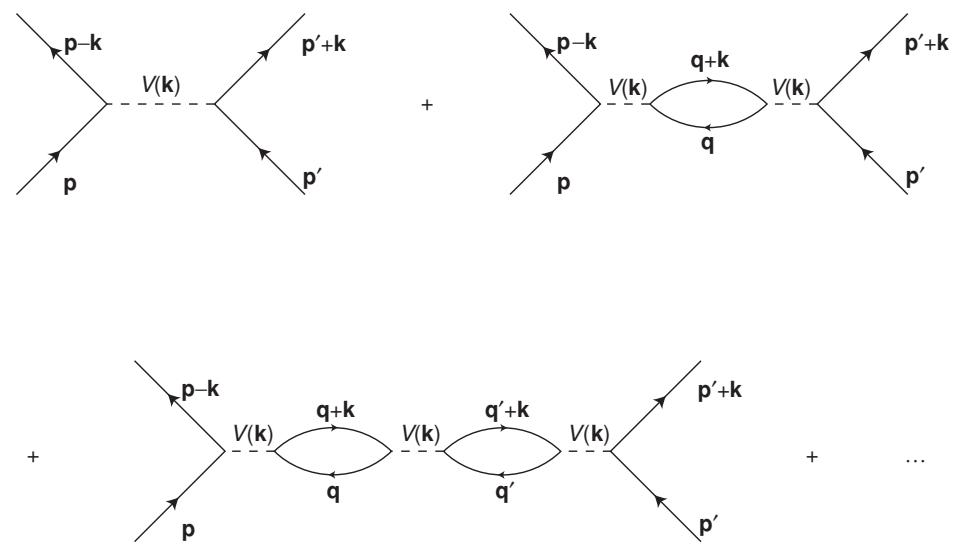
\includegraphics[width=0.8\textwidth]{figs/ch09/fig_9.1.jpg}
\caption*{图 9.1\quad RPA 下屏蔽的电子–电子相互作用的图形展开。每个气泡代表一个粒子–空穴激发。数学上，这些激发由极化函数 $\chi_{nn}^{0}(\mathbf{k},\omega)$ 描述。粒子与空穴之间交换的动量如图所示在各虚线处由库仑相互作用带走。这样一来，库仑相互作用的宗量便与每个气泡中的动量求和脱耦。因此，所有这类项都可以精确求和，其结果即式 (9.82)。}\label{fig:auto:9.1}
\end{figure}

\subsection{结构函数}

上一节定义的含时密度响应函数是多体理论中的一个基本量。除屏蔽函数之外，结构函数（structure function）以及相互作用系统的总能量也都可以用 $\chi_{nn}$ 写出。其主要原因在于，多数多体系统中的势通常是成对相互作用之和。本节集中计算结构函数，因为它将在后面的论题中扮演重要角色。

结构函数定义为粒子密度的傅里叶分量的自关联函数
\begin{equation*}
S(\mathbf{k})=\frac{1}{N}\langle n_{\mathbf{k}}n_{-\mathbf{k}}\rangle\tag{9.85}
\end{equation*}
在平衡态中子散射实验中，所测量的核心量正是结构函数。如前所述，我们也可以用 $S(\mathbf{k},\omega)$ 写出相互作用电子系统的总平均能量。这只需平凡地计算相互作用电子气的哈密顿量在动量空间（见式 (9.18)）中的平均值：
\begin{equation*}
\langle H\rangle=E_0=\epsilon_{\mathrm{kin}}+N\sum_{\mathbf{k}}\frac{2\pi e^2}{k^2}\left[S(\mathbf{k})-1\right].\tag{9.86}
\end{equation*}
在时域中，结构函数变为
\begin{equation*}
S(\mathbf{k},t)=\frac{1}{N}\left\langle\sum_i\mathrm{e}^{\mathrm{i}\mathbf{k}\cdot\mathbf{r}_i(0)}\sum_j\mathrm{e}^{-\mathrm{i}\mathbf{k}\cdot\mathbf{r}_j(t)}\right\rangle.\tag{9.87}
\end{equation*}
注意到
\begin{equation*}
\mathrm{e}^{\mathrm{i}\mathbf{k}\cdot\mathbf{r}_i}=\int\mathrm{d}\mathbf{r}\,\mathrm{e}^{\mathrm{i}\mathbf{k}\cdot\mathbf{r}}\,\delta(\mathbf{r}-\mathbf{r}_i)\tag{9.88}
\end{equation*}
以及 $\mathbf{r}$ 处的密度为
\begin{equation*}
n(\mathbf{r})=\sum_{i=1}^{N}\delta(\mathbf{r}-\mathbf{r}_i),\tag{9.89}
\end{equation*}
便可把式 (9.87) 改写为
\begin{equation*}
S(\mathbf{k},t)=\frac{1}{N}\int\mathrm{d}\mathbf{r}\,\mathrm{d}\mathbf{r}^{\prime}\,\langle n(\mathbf{r},t=0)n(\mathbf{r}^{\prime},t)\rangle\,\mathrm{e}^{\mathrm{i}\mathbf{k}\cdot(\mathbf{r}-\mathbf{r}^{\prime})}.\tag{9.90}
\end{equation*}
如前所见，$\langle n(\mathbf{r},t)n(\mathbf{r}^{\prime},t^{\prime})\rangle$ 只依赖于 $\mathbf{r}-\mathbf{r}^{\prime}$ 和 $t-t^{\prime}$。因此，把时间原点选在 $t=0$ 并不影响结果。动态结构因子（dynamic structure factor）是 $S(\mathbf{k},t)$ 的时间傅里叶变换
\begin{equation*}
S(\mathbf{k},\omega)=\int_{-\infty}^{\infty}\mathrm{d}t\,\mathrm{e}^{-\mathrm{i}\omega t}\,S(\mathbf{k},t),\tag{9.91}
\end{equation*}
在角分辨 X 射线或中子散射实验中测得的正是 $S(\mathbf{k},\omega)$。静态与动态结构因子通过简单的求和规则
\begin{equation*}
S(\mathbf{k})=\int_{-\infty}^{\infty}\frac{\mathrm{d}\omega}{2\pi}\,S(\mathbf{k},\omega).\tag{9.92}
\end{equation*}
相联系。对具有空间反演对称性的系统，例如大多数固体和所有流体，$S(\mathbf{k},\omega)$ 在 $\mathbf{k}$ 变号下不变：$S(\mathbf{k},\omega)=S(-\mathbf{k},\omega)$。由式 (9.59) 可得 $S(\mathbf{k},\omega)=\mathrm{e}^{\beta\hbar\omega}S(\mathbf{k},-\omega)$。这一关系反映细致平衡（detailed balance）原理。

由式 (9.63) 有
\begin{equation*}
\begin{aligned}
\mathrm{i}\hbar\,\chi_{nn}(\mathbf{k},\omega)&=n_{\mathrm{e}}\int_{-\infty}^{0}\mathrm{d}t\,\mathrm{e}^{-\mathrm{i}\omega t}\int_{-\infty}^{\infty}\frac{\mathrm{d}\omega^{\prime}}{2\pi}\,\mathrm{e}^{\mathrm{i}\omega^{\prime}t}\left[S(\mathbf{k},\omega^{\prime})-S(\mathbf{k},-\omega^{\prime})\right]\\
&=n_{\mathrm{e}}\int_{-\infty}^{\infty}\frac{\mathrm{d}\omega^{\prime}}{2\pi\mathrm{i}}\,\frac{S(\mathbf{k},\omega^{\prime})-S(\mathbf{k},-\omega^{\prime})}{\omega^{\prime}-\omega}\\
&=n_{\mathrm{e}}\int_{-\infty}^{\infty}\frac{\mathrm{d}\omega^{\prime}}{2\pi\mathrm{i}}\left(1-\mathrm{e}^{-\beta\hbar\omega^{\prime}}\right)\frac{S(\mathbf{k},\omega^{\prime})}{\omega^{\prime}-\omega}.
\end{aligned}\tag{9.93}
\end{equation*}
由此可见，一旦知道 $S(\mathbf{k},\omega)$，密度响应函数 $\chi_{nn}(\mathbf{k},\omega)$ 原则上便可由实验确定。

\subsection{总能量的参数微分}

用参数微分可以导出与式 (9.86) 相同的表达式。我们考虑基态能量对 $e^2$ 的变分：
\begin{equation*}
\begin{aligned}
\frac{\partial}{\partial e^2}\,E_0(e^2)&=\frac{\partial}{\partial e^2}\langle\psi(e^2)|H|\psi(e^2)\rangle\\
&=\left(\frac{\partial}{\partial e^2}\langle\psi(e^2)|\right)H|\psi(e^2)\rangle+\langle\psi(e^2)|H\left(\frac{\partial}{\partial e^2}|\psi(e^2)\rangle\right)+\langle\psi(e^2)|\frac{\partial H}{\partial e^2}|\psi(e^2)\rangle\\
&=E_0(e^2)\,\frac{\partial}{\partial e^2}\langle\psi(e^2)|\psi(e^2)\rangle+\left\langle\frac{\partial H}{\partial e^2}\right\rangle=\left\langle\psi\left|\frac{\partial H}{\partial e^2}\right|\psi\right\rangle.
\end{aligned}\tag{9.94}
\end{equation*}
其中用到了 $H|\psi(e^2)\rangle=E_0|\psi(e^2)\rangle$ 这一事实。因为动能与 $e^2$ 无关，而 $V\sim e^2$，我们有
\begin{equation*}
\frac{\partial E_0}{\partial e^2}=\frac{1}{e^2}\langle\psi|V_{\mathrm{e}}|\psi\rangle,\tag{9.95}
\end{equation*}
其中 $V_{\mathrm{e}}$ 是我们这个相互作用系统的总势能：
\begin{equation*}
\begin{aligned}
V_{\mathrm{e}}&=V_{\mathrm{ee}}+V_{\mathrm{ion-ion}}+V_{\mathrm{e-ion}}\\
&=e^2\left[\frac{1}{2}\sum_{j,j^{\prime}}\frac{1}{|\mathbf{r}_j-\mathbf{r}_{j^{\prime}}|}+\frac{1}{2}\int\mathrm{d}\mathbf{r}\,\mathrm{d}\mathbf{r}^{\prime}\,\frac{n_{\mathrm{e}}^2}{|\mathbf{r}-\mathbf{r}^{\prime}|}-\sum_j\int\mathrm{d}\mathbf{r}\,\frac{n_{\mathrm{e}}}{|\mathbf{r}-\mathbf{r}_j|}\right].
\end{aligned}\tag{9.96}
\end{equation*}
总势中的第二、三项分别代表离子–离子相互作用和电子–离子相互作用。离子为电子气提供了补偿正电荷的均匀背景。若代入式 (9.89) 的密度形式，可以把总势改写为
\begin{equation*}
\begin{aligned}
\frac{V_{\mathrm{e}}}{e^2}&=\frac{1}{2}\int\mathrm{d}\mathbf{r}\,\mathrm{d}\mathbf{r}^{\prime}\,\frac{n(\mathbf{r})n(\mathbf{r}^{\prime})}{|\mathbf{r}-\mathbf{r}^{\prime}|}+\frac{n_{\mathrm{e}}^2}{2}\int\frac{\mathrm{d}\mathbf{r}\,\mathrm{d}\mathbf{r}^{\prime}}{|\mathbf{r}-\mathbf{r}^{\prime}|}-n_{\mathrm{e}}\int\mathrm{d}\mathbf{r}\,\mathrm{d}\mathbf{r}^{\prime}\,\frac{n(\mathbf{r}^{\prime})}{|\mathbf{r}-\mathbf{r}^{\prime}|}\\
&=\frac{1}{2}\int\mathrm{d}\mathbf{r}\,\mathrm{d}\mathbf{r}^{\prime}\,\frac{(n(\mathbf{r})-n_{\mathrm{e}})\left(n(\mathbf{r}^{\prime})-n_{\mathrm{e}}\right)}{|\mathbf{r}-\mathbf{r}^{\prime}|}.
\end{aligned}\tag{9.97}
\end{equation*}
于是
\begin{equation*}
\begin{aligned}
\frac{\partial E_0}{\partial e^2}&=\frac{1}{2}\int\mathrm{d}\mathbf{r}\,\mathrm{d}\mathbf{r}^{\prime}\,\frac{\langle\delta n(\mathbf{r})\,\delta n(\mathbf{r}^{\prime})\rangle}{|\mathbf{r}-\mathbf{r}^{\prime}|}\\
&=\frac{n_{\mathrm{e}}}{2}\int\mathrm{d}\mathbf{r}\,\mathrm{d}\mathbf{r}^{\prime}\int\frac{\mathrm{d}\mathbf{k}}{(2\pi)^3}\,\frac{\mathrm{e}^{\mathrm{i}\mathbf{k}\cdot(\mathbf{r}-\mathbf{r}^{\prime})}}{|\mathbf{r}-\mathbf{r}^{\prime}|}\int_{-\infty}^{\infty}\frac{\mathrm{d}\omega}{2\pi}\,\tilde{S}(k,\omega)\\
&=\frac{n_{\mathrm{e}}V}{2}\int\frac{\mathrm{d}\mathbf{k}}{(2\pi)^3}\,\frac{4\pi}{k^2}\int_{-\infty}^{\infty}\frac{\mathrm{d}\omega}{2\pi}\,\tilde{S}(k,\omega),
\end{aligned}\tag{9.98}
\end{equation*}
其中我们引入了重新标度的结构因子
\begin{equation*}
n_{\mathrm{e}}\,\tilde{S}(\mathbf{k},\omega)=\int_{-\infty}^{\infty}\mathrm{d}t\,\mathrm{e}^{-\mathrm{i}\omega t}\,\mathrm{e}^{-\mathrm{i}\mathbf{k}\cdot(\mathbf{r}-\mathbf{r}^{\prime})}\,\langle\delta n(\mathbf{r})\,\delta n(\mathbf{r}^{\prime},t)\rangle\,\mathrm{d}(\mathbf{r}-\mathbf{r}^{\prime}).\tag{9.99}
\end{equation*}
结构因子这一定义的优点是消除了能量中通常会出现的 $n_{\mathrm{e}}^2$ 项。\footnote{译注：式 (9.99) 末尾原书即印作 $\mathrm{d}(\mathbf{r}-\mathbf{r}^{\prime})$，按上下文其前疑脱积分号，应为对 $\mathbf{r}-\mathbf{r}^{\prime}$ 的空间积分。}这一项只是移动势能的零点，因而并无实质影响。对 $S(\mathbf{k},\omega)$ 使用式 (9.92) 的求和规则，得到
\begin{equation*}
E_0(e^2)=E_0(e^2=0)+\frac{N}{2}\int_{0}^{e^2}\mathrm{d}e^{\prime 2}\int\frac{\mathrm{d}\mathbf{k}}{(2\pi)^3}\,\frac{4\pi}{k^2}\,\tilde{S}(\mathbf{k};e^{\prime 2}),\tag{9.100}
\end{equation*}
其中我们允许静态结构因子显式地依赖 $e^2$。这是一个精确表达式。若 $\tilde{S}(\mathbf{k})$ 取自由粒子形式，得到的就是哈特里–福克理论。再纳入屏蔽效应，便可以把 $E_0(e^2)$ 归约到盖尔曼–布吕克纳（Gell-Mann--Brueckner）微扰展开。

\subsection{$\chi_{\mathrm{sc}}(\mathbf{k},\omega)$ 的计算}

我们现在的目标是在 RPA 中把屏蔽效应完全求出。先把屏蔽函数改写为
\begin{equation*}
\begin{aligned}
\chi_{\mathrm{sc}}(\mathbf{k},\omega)&=\chi_{nn}^{0}(\mathbf{k},\omega)=2\int\frac{\mathrm{d}\mathbf{p}}{(2\pi\hbar)^3}\,\frac{\left(f_{\mathbf{p}}-f_{\mathbf{p}+\hbar\mathbf{k}}\right)}{\left(\hbar\omega+\epsilon_{\mathbf{p}}-\epsilon_{\mathbf{p}+\hbar\mathbf{k}}\right)}\\
&=2\lim_{\eta\to 0}\int_{-\infty}^{\infty}\frac{\mathrm{d}\omega^{\prime}}{\omega-\omega^{\prime}+\mathrm{i}\eta}\int\frac{\mathrm{d}\mathbf{p}}{(2\pi\hbar)^3}\left(f_{\mathbf{p}}-f_{\mathbf{p}+\hbar\mathbf{k}}\right)\delta(\hbar\omega^{\prime}-\epsilon_{\mathbf{p}+\hbar\mathbf{k}}+\epsilon_{\mathbf{p}}).
\end{aligned}\tag{9.101}
\end{equation*}
利用式 (9.93)，把右边用结构因子改写，得到
\begin{equation*}
4\pi\hbar\int\frac{\mathrm{d}\mathbf{p}}{(2\pi\hbar)^3}\left(f_{\mathbf{p}}-f_{\mathbf{p}+\hbar\mathbf{k}}\right)\delta(\hbar\omega^{\prime}-\epsilon_{\mathbf{p}+\hbar\mathbf{k}}+\epsilon_{\mathbf{p}})=n_{\mathrm{e}}\left(1-\mathrm{e}^{-\beta\hbar\omega^{\prime}}\right)S_0(k,\omega^{\prime}),
\end{equation*}
其中 $S_0(\mathbf{k},\omega^{\prime})$ 是自由系统的结构因子。注意到 $f_{\mathbf{p}}-f_{\mathbf{p}+\hbar\mathbf{k}}=f_{\mathbf{p}}(1-f_{\mathbf{p}+\hbar\mathbf{k}})-f_{\mathbf{p}+\hbar\mathbf{k}}(1-f_{\mathbf{p}})$ 以及 $1-f_{\mathbf{p}}=\mathrm{e}^{\beta(\epsilon_{\mathbf{p}}-\mu)}f_{\mathbf{p}}$，可以简化此表达式的左边。于是
\begin{equation*}
f_{\mathbf{p}}-f_{\mathbf{p}+\hbar\mathbf{k}}=f_{\mathbf{p}}\left(1-f_{\mathbf{p}+\hbar\mathbf{k}}\right)\left(1-\mathrm{e}^{\beta(\epsilon_{\mathbf{p}}-\epsilon_{\mathbf{p}+\hbar\mathbf{k}})}\right),\tag{9.102}
\end{equation*}
乘在自由粒子结构函数上的显式温度依赖因子便可以消去，得到
\begin{equation*}
n_{\mathrm{e}}S_0(\mathbf{k},\omega)=4\pi\hbar\int\frac{\mathrm{d}\mathbf{p}}{(2\pi\hbar)^3}\,f_{\mathbf{p}}\left(1-f_{\mathbf{p}+\hbar\mathbf{k}}\right)\delta(\hbar\omega-\epsilon_{\mathbf{p}+\hbar\mathbf{k}}+\epsilon_{\mathbf{p}}).\tag{9.103}
\end{equation*}
因子 $1-f_{\mathbf{p}+\hbar\mathbf{k}}$ 是动量为 $\mathbf{p}+\hbar\mathbf{k}$ 的态空着的概率。因此，$S_0(\mathbf{k},\omega)$ 由粒子与空穴交换能量（总能量变化为 $\hbar\omega=\epsilon_{\mathbf{p}}-\epsilon_{p+\hbar\mathbf{k}}$）的方式数决定。在这个意义上，可以把 $S_0(\mathbf{k},\omega)$ 看作粒子–空穴激发的有效态密度。

为在 $T=0$ 下计算式 (9.103) 中的积分，把 $f_{\mathbf{p}+\hbar\mathbf{k}}$ 中的动量平移 $-\hbar\mathbf{k}$，所得被积函数
\begin{equation*}
\begin{aligned}
2\int\frac{\mathrm{d}\mathbf{p}}{(2\pi\hbar)^2}\left(f_{\mathrm{p}}-f_{\mathrm{p}+\hbar\mathbf{k}}\right)\delta(\hbar\omega-\epsilon_{\mathrm{p}+\hbar\mathbf{k}}+\epsilon_{\mathrm{p}})&\\
=2\int\frac{\mathrm{d}\mathbf{p}}{(2\pi\hbar)^2}\,f_{\mathrm{p}}\left[\delta(\hbar\omega-\epsilon_{\mathrm{p}+\hbar\mathbf{k}}+\epsilon_{\mathrm{p}})-\delta(\hbar\omega-\epsilon_{\mathrm{p}}+\epsilon_{\mathrm{p}-\hbar\mathbf{k}})\right]&\\
=2\int\frac{\mathrm{d}\mathbf{p}}{(2\pi\hbar)^2}\,f_{\mathrm{p}}\left[\delta\left(\hbar\omega-\frac{(\hbar k)^2}{2m}-\frac{\mathbf{p}\cdot\hbar\mathbf{k}}{m}\right)-\delta\left(\hbar\omega+\frac{(\hbar k)^2}{2m}+\frac{\mathbf{p}\cdot\hbar\mathbf{k}}{m}\right)\right]&\\
=I_{\omega}-I_{-\omega},&
\end{aligned}\tag{9.104}
\end{equation*}
便只含一个费米分布函数。\footnote{译注：式 (9.104) 中三处积分测度均照录原书印出的 $(2\pi\hbar)^2$；按式 (9.103) 应为 $(2\pi\hbar)^3$。}现在变换到球坐标，得到
\begin{equation*}
\begin{aligned}
I_{\omega}&=\frac{1}{\pi\hbar^2}\int_{0}^{p_{\mathrm{F}}}p^2\,\mathrm{d}p\int_{-1}^{1}\mathrm{d}\mu\,\delta\left(\hbar\omega-\frac{(\hbar k)^2}{2m}-\frac{\hbar kp\mu}{m}\right)\\
&=\frac{m}{\pi k\hbar^3}\int_{0}^{p_{\mathrm{F}}}p\,\mathrm{d}p\,\Theta\left(1-\left|\frac{m}{\hbar kp}\left(\hbar\omega-\frac{(\hbar k)^2}{2m}\right)\right|\right)\\
&=\frac{m}{\pi k\hbar^3}\int_{\frac{m}{\hbar k}\left|\hbar\omega-\frac{(\hbar k)^2}{2m}\right|}^{p_{\mathrm{F}}}p\,\mathrm{d}p\\
&=\frac{m}{2\pi k\hbar^3}\left[p_{\mathrm{F}}^2-\left(\frac{m}{\hbar k}\left(\hbar\omega-\frac{(\hbar k)^2}{2m}\right)\right)^{\!2}\right]\Theta\left(p_{\mathrm{F}}-\frac{m}{\hbar k}\left|\hbar\omega-\frac{(\hbar k)^2}{2m}\right|\right)
\end{aligned}\tag{9.105}
\end{equation*}
这里 $\Theta(x)$ 是亥维赛（Heaviside）阶跃函数。减去 $\omega\to-\omega$ 的贡献，得到
\begin{equation*}
\begin{aligned}
I_{\omega}-I_{-\omega}&=\frac{m}{2\pi k\hbar^3}\left[p_{\mathrm{F}}^2-\left(\frac{m}{\hbar k}\left(\hbar\omega-\frac{(\hbar k)^2}{2m}\right)\right)^{\!2}\right]\Theta\left(p_{\mathrm{F}}-\frac{m}{\hbar k}\left|\hbar\omega-\frac{(\hbar k)^2}{2m}\right|\right)\\
&-\frac{m}{2\pi k\hbar^3}\left[p_{\mathrm{F}}^2-\left(\frac{m}{\hbar k}\left(\hbar\omega+\frac{(\hbar k)^2}{2m}\right)\right)^{\!2}\right]\Theta\left(p_{\mathrm{F}}-\frac{m}{\hbar k}\left|\hbar\omega+\frac{(\hbar k)^2}{2m}\right|\right)
\end{aligned}\tag{9.106}
\end{equation*}
亥维赛阶跃函数对第一项施加约束
\begin{equation*}
\frac{(\hbar k)^2}{2m}-\hbar kv_{\mathrm{F}}<\hbar\omega<\frac{(\hbar k)^2}{2m}+\hbar kv_{\mathrm{F}}\tag{9.107}
\end{equation*}
对第二项施加约束
\begin{equation*}
0<\hbar\omega<\hbar kv_{\mathrm{F}}-\frac{(\hbar k)^2}{2m}.\tag{9.108}
\end{equation*}
对 $\omega>0$，这些限制在图 9.2 中以图形表示，其中 $\omega_{\pm}=(\hbar k)^2/2m\pm\hbar kv_{\mathrm{F}}$。

\begin{figure}[H]\centering
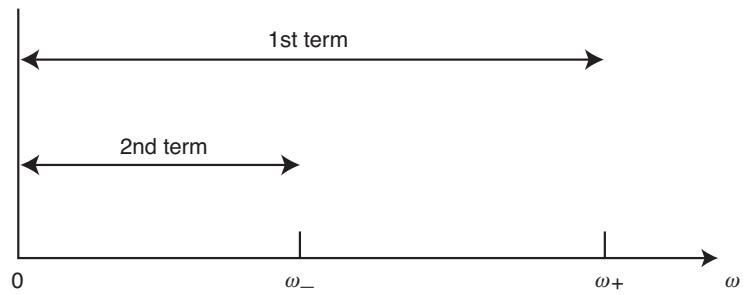
\includegraphics[width=0.5\textwidth]{figs/ch09/fig_9.2.jpg}
\caption*{图 9.2\quad 零温结构函数的频率范围。}\label{fig:auto:9.2}
\end{figure}

\begin{figure}[H]\centering
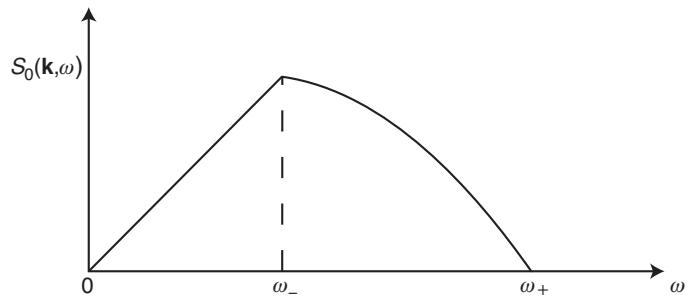
\includegraphics[width=0.5\textwidth]{figs/ch09/fig_9.3.jpg}
\caption*{图 9.3\quad 由式 (9.110–9.112) 预言的零温函数。}\label{fig:auto:9.3}
\end{figure}

由于式 (9.106) 中第一项的 $\omega$ 范围超出第二项的范围，我们分三种情形讨论，分别对应于 (a) 两项都有贡献、(b) 只有第一项、(c) 两者皆无：

情形（a）$0<\hbar\omega<\hbar kv_{\mathrm{F}}-(\hbar k)^2/2m$：
\begin{equation*}
\begin{aligned}
I_{\omega}-I_{-\omega}=n_{\mathrm{e}}S_0(\mathbf{k},\omega)=\frac{m}{2\pi k\hbar^3}\bigg[p_{\mathrm{F}}^2-\left(\frac{m}{\hbar k}\left(\hbar\omega-\frac{(\hbar k)^2}{2m}\right)\right)^{\!2}\qquad&\\
\left.-\left[p_{\mathrm{F}}^2-\left(\frac{m}{\hbar k}\left(\hbar\omega+\frac{(\hbar k)^2}{2m}\right)\right)^{\!2}\right]\right]&
\end{aligned}\tag{9.109}
\end{equation*}
\begin{equation*}
\Rightarrow\; n_{\mathrm{e}}S_0(\mathbf{k},\omega)=\frac{m^2\omega}{\pi\hbar^2 k};\tag{9.110}
\end{equation*}

情形（b）$\hbar kv_{\mathrm{F}}-(\hbar k)^2/2m<\hbar\omega<(\hbar k)^2/2m+\hbar kv_{\mathrm{F}}$：
\begin{equation*}
\Rightarrow\; n_{\mathrm{e}}S_0(\mathbf{k},\omega)=\frac{m}{2\pi k\hbar^3}\left[p_{\mathrm{F}}^2-\left(\frac{m}{\hbar k}\left(\hbar\omega-\frac{(\hbar k)^2}{2m}\right)\right)^{\!2}\right];\tag{9.111}
\end{equation*}

情形（c）$\hbar\omega>\dfrac{(\hbar k)^2}{2m}+\hbar kv_{\mathrm{F}}$：
\begin{equation*}
\Rightarrow\; n_{\mathrm{e}}S_0(\mathbf{k},\omega)=0.\tag{9.112}
\end{equation*}

图 9.3 给出了三种情形合并在一起的图线。

在有限温度下，也能得到 $n_{\mathrm{e}}S_0(\mathbf{k},\omega)$ 的显式表达式。只需计算 $I_{\omega}$，再令 $\omega\to-\omega$。由式 (9.103) 有
\begin{equation*}
\begin{aligned}
\mathrm{I}_{\omega}&=\frac{m}{\pi k\hbar^3}\int_{(1/2\hbar k)\left|2m\hbar\omega-k^2\hbar^2\right|}^{p_{\mathrm{F}}}\frac{p\,\mathrm{d}p}{\mathrm{e}^{\beta(\epsilon_{\mathrm{p}}-\mu)}+1}\\
&=\frac{m^2}{\beta\pi k\hbar^3}\int_{a}^{p_{\mathrm{F}}}\left(\frac{\beta p}{m}\right)\mathrm{d}p\,\frac{1}{\mathrm{e}^{\beta(\epsilon_{\mathrm{p}}-\mu)}+1}\\
&=\frac{m^2}{\beta\pi k\hbar^3}\int_{\beta a^2/2m}^{\beta p_{\mathrm{F}}^2/2m}\frac{\mathrm{d}x}{\mathrm{e}^{x-\beta\mu}+1}.
\end{aligned}\tag{9.113}
\end{equation*}
借助积分
\begin{equation*}
\int\frac{\mathrm{d}x}{1+b\,\mathrm{e}^{cx}}=\frac{1}{c}\left[cx-\ln(1+b\,\mathrm{e}^{cx})\right],\tag{9.114}
\end{equation*}
可得
\begin{equation*}
I_{\omega}=\frac{m^2}{\beta\pi\hbar^3 k}\left[x-\ln(1+\mathrm{e}^{x-\beta\mu})\right]_{\beta a^2/2m}^{\beta p_{\mathrm{F}}^2/2m},\tag{9.115}
\end{equation*}
于是得到依赖温度的结构函数的最终表达式：
\begin{equation*}
\begin{aligned}
\left(1-\mathrm{e}^{-\beta\hbar\omega}\right)n_{\mathrm{e}}S_0(\mathbf{k},\omega)&=I_{\omega}-I_{-\omega}\\
&=\frac{m^2}{\beta\pi\hbar^3 k}\left[\beta\hbar\omega+\ln\left[\frac{1+\exp\left(\beta\left(\frac{1}{2m}\left(\frac{m\omega}{k}-\frac{\hbar k}{2}\right)^{2}-\mu\right)\right)}{1+\exp\left(\beta\left(\frac{1}{2m}\left(\frac{m\omega}{k}+\frac{\hbar k}{2}\right)^{2}-\mu\right)\right)}\right]\right].
\end{aligned}
\end{equation*}
在零温极限下，便回到前面在 $T=0$ 时导出的表达式。

\subsection{介电函数}

现在转向介电响应函数 $\varepsilon(\mathbf{k},\omega)=1-4\pi e^2\chi_{\mathrm{sc}}(\mathbf{k},\omega)/k^2$ 的计算，其中 RPA 层次的屏蔽函数
\begin{equation*}
\chi_{\mathrm{sc}}(\mathbf{k},\omega)=\lim_{\eta\to 0}\int_{-\infty}^{\infty}\frac{\mathrm{d}\omega^{\prime}}{2\pi\hbar}\,\frac{n_{\mathrm{e}}S_0(\mathbf{k},\omega^{\prime})\left(1-\mathrm{e}^{-\beta\hbar\omega^{\prime}}\right)}{\omega-\omega^{\prime}+\mathrm{i}\eta},\tag{9.116}
\end{equation*}
是结构函数的卷积。在 $\eta\to 0$ 的极限下，屏蔽函数将通过
\begin{equation*}
\lim_{\eta\to 0}\frac{1}{\omega-\omega^{\prime}+\mathrm{i}\eta}=P\,\frac{1}{\omega-\omega^{\prime}}-\mathrm{i}\pi\delta(\omega^{\prime}-\omega).\tag{9.117}
\end{equation*}
获得实部和虚部。介电函数相应的实部与虚部分别为
\begin{equation*}
\varepsilon_{\mathrm{R}}(\mathbf{k},\omega)=1-\frac{4\pi e^2}{k^2}\,P\int_{-\infty}^{\infty}\frac{\mathrm{d}\omega^{\prime}}{2\pi\hbar}\,\frac{n_{\mathrm{e}}S_0(\mathbf{k},\omega^{\prime})\left(1-\mathrm{e}^{-\beta\hbar\omega^{\prime}}\right)}{(\omega-\omega^{\prime})}\tag{9.118}
\end{equation*}
与
\begin{equation*}
\varepsilon_{\mathrm{I}}=\frac{2\pi e^2}{k^2\hbar}\,n_{\mathrm{e}}S_0(\mathbf{k},\omega)\left(1-\mathrm{e}^{-\beta\hbar\omega}\right),\tag{9.119}
\end{equation*}

\begin{figure}[H]\centering
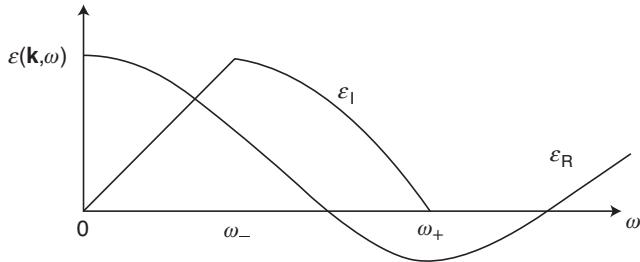
\includegraphics[width=0.55\textwidth]{figs/ch09/fig_9.4.jpg}
\caption*{图 9.4\quad $T=0$ 时介电函数的实部（$\varepsilon_{\mathrm{R}}$）与虚部（$\varepsilon_{\mathrm{I}}$）。}\label{fig:auto:9.4}
\end{figure}

在零温极限下，$S_0(\mathbf{k},\omega)$ 对频率是线性的，因此 $\varepsilon_{\mathrm{I}}$ 是频率的奇函数。

由于对试探电荷的响应具有因果性，介电函数的实部和虚部是相互关联的。不过这里要小心：介电函数中只有与 $\chi_{\mathrm{sc}}$ 直接相关的部分才表现出因果响应。也就是说，$\varepsilon_{\mathrm{R}}-1$，
\begin{equation*}
\varepsilon_{\mathrm{R}}-1=\frac{1}{\pi}\,P\int_{-\infty}^{\infty}\frac{\mathrm{d}\omega^{\prime}\,\varepsilon_{\mathrm{I}}(\mathbf{k},\omega^{\prime})}{\omega^{\prime}-\omega},\tag{9.120}
\end{equation*}
与 $\varepsilon_{\mathrm{I}}$，
\begin{equation*}
\varepsilon_{\mathrm{I}}=\frac{-P}{\pi}\int_{-\infty}^{\infty}\frac{\mathrm{d}\omega^{\prime}\,\varepsilon_{\mathrm{R}}(\mathbf{k},\omega^{\prime})-1}{\omega^{\prime}-\omega},\tag{9.121}
\end{equation*}
通过克拉默斯–克勒尼希（Kramers--Kronig）关系相联系。正如第 7 章格林函数一节所见，这类关系对任一在上半平面或下半平面解析的复函数普遍成立。在线性响应理论的语境中，它们从根本上源于对含时微扰之响应的因果性。

林哈德（Lindhard）(L1954) 证明，在 $T=0$ 时 $\varepsilon_{\mathrm{R}}$ 为
\begin{equation*}
\begin{aligned}
\varepsilon_{\mathrm{R}}&=1+\frac{\kappa_{\mathrm{TF}}^2}{k^2}\left\{\frac{1}{2}+\frac{k_{\mathrm{F}}}{4k}\left[\left\{1-\frac{\left(\omega-\hbar k^2/2m\right)^2}{k^2v_{\mathrm{F}}^2}\right\}\ln\left|\frac{\omega-kv_{\mathrm{F}}-\hbar k^2/2m}{\omega+kv_{\mathrm{F}}-\hbar k^2/2m}\right|\right.\right.\\
&\qquad\left.\left.+\left\{1-\frac{\left(\omega+\hbar k^2/2m\right)^2}{k^2v_{\mathrm{F}}^2}\right\}\ln\left|\frac{\omega+kv_{\mathrm{F}}+\hbar k^2/2m}{\omega-kv_{\mathrm{F}}+\hbar k^2/2m}\right|\right]\right\}.
\end{aligned}\tag{9.122}
\end{equation*}
首先注意，此函数与 $\omega$ 的符号无关，因此其奇偶性与 $\varepsilon_{\mathrm{I}}$ 相反。介电函数的一般频率依赖如图 9.4 所示。$\omega\to 0$ 时 $\varepsilon_{\mathrm{R}}$ 的巨大数值表明静态屏蔽很强。介电响应函数的另一个特征是，在等离体频率处 $\varepsilon(\mathbf{k},\omega)=0$。$\varepsilon^{-1}(\mathbf{k},\omega)$ 的极点出现在电子气的激发频率处。回想一下，这正是我们前面在介电函数的小 $k$、大 $\omega$ 展开中导出的结果。当 $\varepsilon(\mathbf{k},\omega)=0$ 时，由于等离体振荡的集体性质，电子密度的涨落发散。在这一点上，我们建立的整个理论都失效了，因为我们曾假设电子密度是微扰场的缓变函数。让我们考察 $\varepsilon(\mathbf{k},\omega)$ 在小 $\omega$ 下的行为。在 $\varepsilon_{\mathrm{R}}$ 的表达式中令 $\omega=0$，得到
\begin{equation*}
\varepsilon(x,\omega=0)=\varepsilon_{\mathrm{R}}(x,\omega=0)=1+\frac{\kappa_{\mathrm{TF}}^2}{k^2}\left[\frac{1}{2}+\frac{1-x^2}{4x}\,\ln\left|\frac{1+x}{1-x}\right|\right],\tag{9.123}
\end{equation*}
即静态极限下的介电函数，其中 $x=k/2k_{\mathrm{F}}$。$\varepsilon(x,\omega=0)=1+\kappa_{\mathrm{TF}}^2/k^2$ 在 $x=0$ 处的极限，正是对原点处正电荷之屏蔽的托马斯–费米近似。

与托马斯–费米情形一样，我们可以构造出由这类屏蔽效应导致的空间电势。为此，利用有效场的方程 $U_{\mathrm{eff}}(k,\omega)=\varepsilon^{-1}(\mathbf{k},\omega)U(\mathbf{k},\omega)$。对电子气，$U(\mathbf{k},\omega=0)=4\pi e^2/k^2$。若用 $\varepsilon(\mathbf{k},\omega=0)$ 的表达式，我们发现
\begin{equation*}
\phi_{\mathrm{eff}}(\mathbf{r})=4\pi e\int\frac{\mathrm{d}\mathbf{k}}{(2\pi)^3}\,\frac{\mathrm{e}^{-\mathrm{i}\mathbf{k}\cdot\mathbf{r}}}{k^2+\kappa_{\mathrm{TF}}^2\,Q(\mathbf{k})}\tag{9.124}
\end{equation*}
就是有效电势的空间依赖，其中 $Q(\mathbf{k})$ 表示式 (9.123) 中方括号项的傅里叶变换。当 $k=2k_{\mathrm{F}}$ 时，$Q(\mathbf{k})$ 对数发散。这一发散使静电势获得如下形式的贡献
\begin{equation*}
\phi_{\mathrm{eff}}\sim\frac{\cos 2k_{\mathrm{F}}r}{r^3}\tag{9.125}
\end{equation*}
（当 $r\to\infty$ 时）。静电势的这种振荡行为纯粹是屏蔽的后果，称为弗里德德尔振荡（Friedel oscillation）(F1954)。于是在长距离处，我们发现电荷并未被充分屏蔽到给出托马斯–费米理论的 $\mathrm{e}^{-\kappa_{\mathrm{TF}}r}/r$ 形式。静电势的代数式衰减意味着，一个局域的外电荷会影响到电子气中各处的电荷密度。科恩（Kohn）(K1959) 最先论证，屏蔽静电势的这种缓慢衰减源于费米面的锐利。对净动量转移 $k>2k_{\mathrm{F}}$ 的激发，这一效应会显现于金属的声子谱中。他还与卢廷格（Luttinger）一起指出 (KL1965)，$\phi_{\mathrm{eff}}$ 的负值贡献会在 $T=0$ 的电子气中导致超导不稳定性。这一论断意义重大，因为它表明：任其自然的话，具有裸排斥相互作用的电子气无须声子协助也能变为超导。
